\documentclass[11pt,a4paper,titlepage]{article}
\usepackage[pdftex]{graphicx}
\usepackage{listings}
\usepackage{titlesec}
\usepackage{float}
\usepackage{enumitem}
\usepackage{color}
\usepackage{pdflscape}
\usepackage{algpseudocode}
\usepackage{algorithm}
\usepackage{hyperref}
\hypersetup{
	colorlinks,
	citecolor=black,
	filecolor=black,
	linkcolor=black,
	urlcolor=black
}

\setcounter{secnumdepth}{4}

\titleformat{\paragraph}
{\normalfont\normalsize\bfseries}{\theparagraph}{1em}{}
\titlespacing*{\paragraph}
{0pt}{3.25ex plus 1ex minus .2ex}{1.5ex plus .2ex}

\begin{document}
\begin{figure}
	\centering
	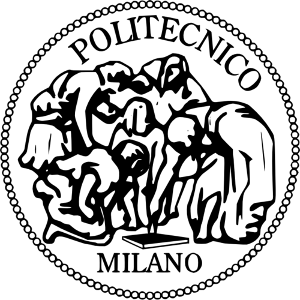
\includegraphics[scale=0.6]{../SE2_IMAGES/Logo_Politecnico_Milano}
\end{figure}
\title{Politecnico di Milano\\A.Y. 2015/2016\\\textbf{My Taxi Service}\\Design Document\\}
\author{Bernardis Cesare matr. 852509 \and Dagrada Mattia matr.852975}
\date{December 4, 2015}
\maketitle

\newpage

\tableofcontents

\newpage

\section{Introduction}
\subsection{Purpose}
The main goal of this document is to completely describe the system in terms of functional and non-functional requirements, to analyse the real need of the customer modelling the system, to show the constraints and the software limits and simulate the typical use cases that will occur after the development. This document is intended to all developers and programmers who have to implement the requirements, to the system analysts who want to integrate other system with this one, and could also be used as a contractual basis between the customer and the developer.
\subsection{Actual system}
The government of a large city wants to optimize its taxi service. We suppose that the actual taxi service is based on simple phone calls from customers to the taxi's call centre.
\subsection{Scope}
The aim of this project is to create a brand new taxi application that is used by both the taxi drivers and the passengers to access the taxi service. Passengers can access the service either via mobile or web application. They can request a taxi without having to register to service but they have to insert personal information while registered passengers, once logged in, can directly request a taxi. The system confirms a taxi request by sending the passenger the taxi code only when a taxi is found and an estimated arrival time. Registered passengers can also make taxi reservations and they will receive the code as soon as a taxi is found available. Taxi drivers can access the service only from mobile application. Once logged in they can give the system their availability, or revoke it, and they will receive from the system ride requests that they can either accept or refuse. The login interface of the application is shared by passengers and taxi drivers.
The system has the city map divided into areas of 2km$^{2}$ and holds a taxi queue in each area. It receives GPS coordinates from taxis, it assigns them to their corresponding area queue, placing them in the last position. Following a FIFO (First In First Out) logic, the first taxi receives a request and is then removed from the queue. In case of rejection, the taxi is placed in the last position of the queue.
\subsection{Actors}
\begin{description}
	\item[Guest] a guest is able to request a taxi without having to be registered to the service, but simply adding some essential personal information. A guest can register to the service filling in a registration form, becoming a Registered Passenger.
	\item[Registered Passenger] a registered passenger, once logged in, is able to request a taxi without having to add additional personal information. A registered passenger can also make reservations, specifying origin and destination of the ride, at least 2 hours before the desired time for the ride.
	\item[Taxi Drivers] a taxi driver, once logged in, has a different user interface than registered user, from which he will receive ride requests that he can accept or refuse. He will also be able to give his availability, which means that he is willing to pick up ride requests.
\end{description}
\subsection{Goals}
These are the goals of MyTaxiService application:
\begin{itemize}
	\item Permit a guest to register to the service.
	\item Permit a guest to request a taxi.
	\item Permit a guest to sign in and become a registered passenger
	\item Permit a registered passenger to require a taxi.
	\item Permit a registered passenger to make a reservation.
	\item Permit a registered passenger to cancel a reservation.
	\item Permit a taxi driver to give the system his availability.
	\item Permit a taxi driver to revoke his availability.
	\item Permit a taxi driver to accept a ride request.
	\item Permit a taxi driver to refuse a ride request.
\end{itemize}
\subsection{Reference Documents}
\begin{itemize}
	\item Specification Document: MyTaxiService Project A.Y.2015-2016.
	\item IEEE Std 830-1998 IEEE Recommended Practice for Software Requirements Specifications.
\end{itemize}
\subsection{Document overview}
This document is structured as following:
\begin{enumerate}
	\item \textbf{Introduction}: this section represents a generic description of the project, highlighting actors and goals.
	\item \textbf{Overall Description}: this section gives further informations about the project, focusing more on what are the assumptions made about the software and its constraints.
	\item \textbf{Specific Requirements}: this section lists the requirements of the software, both functional and non-functional ones. There are also some typical scenarios and use cases related to sequence diagrams along with a class diagram.
	\item \textbf{Alloy Modelling}: this section contains Alloy code and Alloy worlds.
	\item \textbf{Appendix}: this section contains extra information and also which software and tools has been used to write this document.
\end{enumerate}
\section{Architectural Design}
	\subsection{Overview}
	In this section we will talk about the system in its complex. We will show how we think that it should
	work, in particular we will present which should be its structure, the most important components and
	how they interact each other. We thought our system with a four tier architecture, in order to be compatible
	with a JEE Architecture implementation.
	\begin{figure}[h!]
		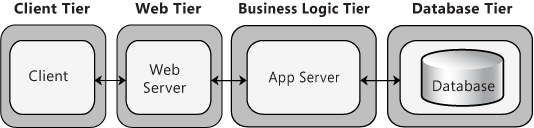
\includegraphics[width=\linewidth]{../SE2_IMAGES/4tier}
		\caption{Four tier architecture}
	\end{figure}
	\newline
	However, we do not want to limit the ways it could be implemented, so
	we will present the JEE as an example, \textbf{not as a constraint}. JEE is useful because provides some services
	"on the shelf" (ready to use) and we recommend to reuse the existing code to avoid a useless waste of time,
	but the possibility is always open for a more specific, and performing, implementation of the system.
	\clearpage
	\begin{figure}[h!]
		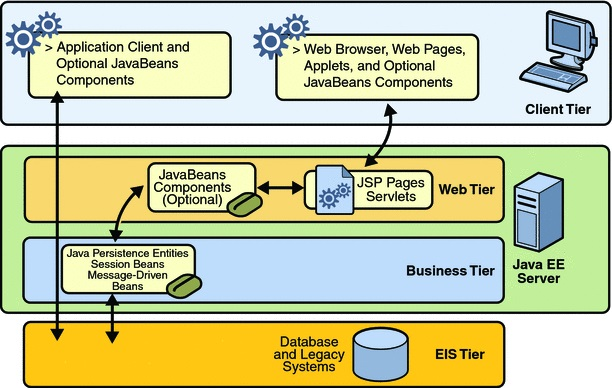
\includegraphics[width=\linewidth]{../SE2_IMAGES/jee}
		\caption{Java Enterprise Edition architecture}
	\end{figure}
	\begin{description}
		\item[Client tier] contains Application Clients and Web Browsers and it is the layer that interacts
		directly with the actors. In our case this tier contains both of them, because we have a usual web
		application and a mobile app.
		\item[Web tier] contains the Servlets and Dynamic Web Pages that needs to be elaborated. It could
		also include some optional JavaBeans. This tier receives the requests from the client tier and forwards
		the pieces of data collected to the business tier waiting for processed data to be sent
		to the client tier correctly formatted
		\item[Business tier] contains the Java Beans (the business logic of the application)	and Java
		Persistence Entities which represent the physical data of the system.
		\item[EIS tier] contains the persistent data source and destination.	It is another way to refer
		to the database of our system.
	\end{description}
	\newpage
	\subsection{High Level Components and their interaction}
	\label{subsec:High Level Components and their interaction}
	We start introducing how we thought the four tier architecture of our system.
	\begin{figure}[h!]
		\begin{center}
			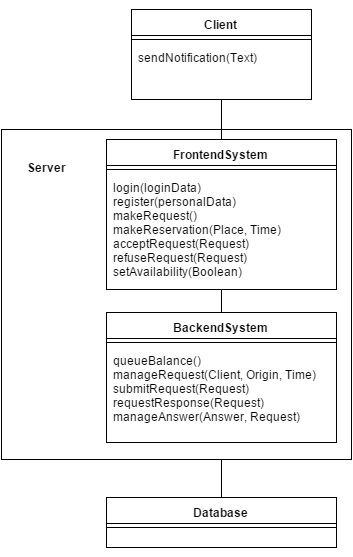
\includegraphics[height=0.5\textheight]{../SE2_IMAGES/HLC}
			\caption{High Level Component representation}
		\end{center}
	\end{figure}
	The top block represents the Client, where the application or the web browser runs with our	clients.
	The Client is connected to the Server of our application, which is divided in two subsystems:
	\begin{description}
		\item[Frontend] which represents the part of our system that provides to the client all the necessary
		functions to perform all the functionalities that are required by the application
		\item[Backend] which represents the beating hearth of our system, where all the requests, reservations,
		and the services that our system should provide, are created and maintained.
	\end{description}
	The end point is the Database, where all the persistent data is stored for a long term availability.
	\newpage
	\begin{landscape}
	\subsection{Component view}
	This is a diagram that represents the whole system. We are focusing on the global components and their
	connections, providing also a preview of the interfaces that the various components provide for the
	interaction. A more detailed explanation of the single components follows the diagram.
		\begin{figure}[h!]
			\begin{center}
				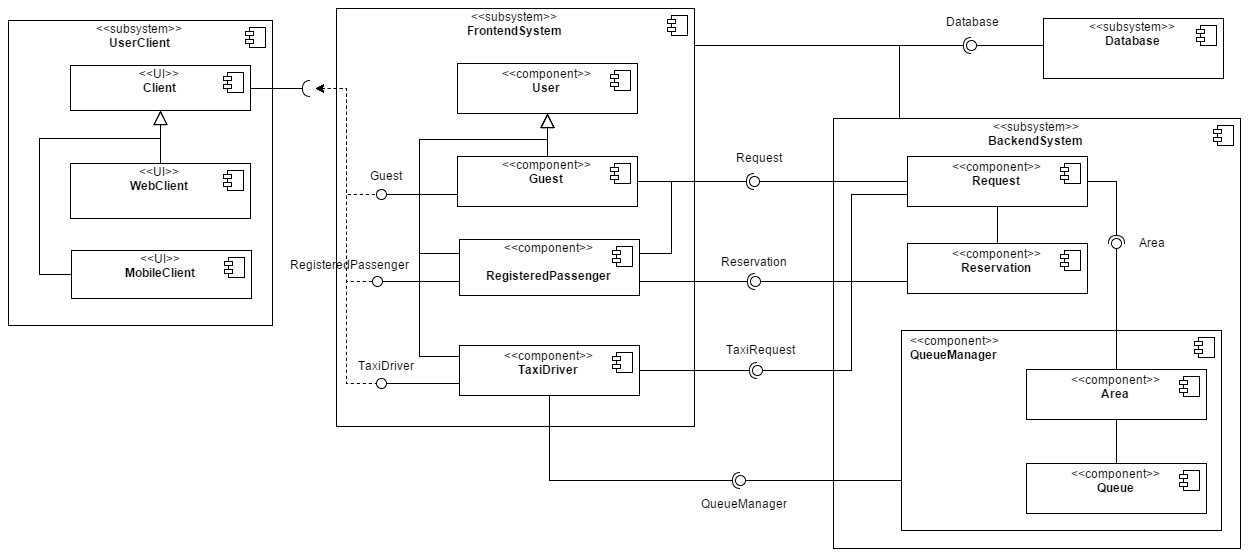
\includegraphics[width=0.9\linewidth]{../SE2_IMAGES/ComponentDiagram}
				\caption{Component Diagram}
			\end{center}
		\end{figure}
	\end{landscape}
	\newpage
	\subsubsection{Client}
		\begin{figure}[h!]
			\begin{center}
				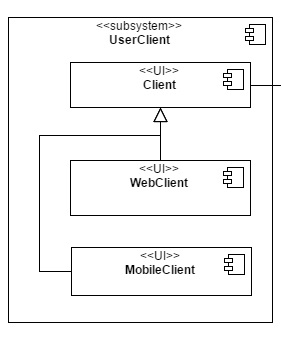
\includegraphics[scale=1]{../SE2_IMAGES/UserClient}
				\caption{Client components}
			\end{center}
		\end{figure}
		In this subsystem we have the components in direct contact with the user.
		It can be considered the user's "access interface" of our system.
		\paragraph{Client} user interface represents the generic type of client that interact with the system. It will most likely be an abstract class extended by WebClient and MobileClient.
		\paragraph{WebClient, MobileClient} user interfaces represent a generalization of the Client since they both share the same functionalities except for the fact that a Taxi Driver can only use the MobileClient to interact with the system. They main difference between these two user interfaces is the different type of communication protocols they use to interact with the system.
	\subsubsection{Frontend}
		\begin{figure}[h!]
			\begin{center}
				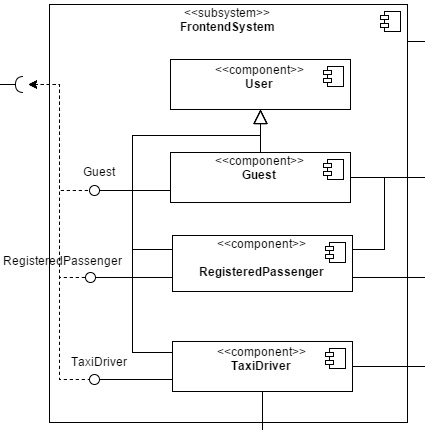
\includegraphics[width=1\linewidth]{../SE2_IMAGES/Frontend}
				\caption{Backend components}
			\end{center}
		\end{figure}
		This subsystem represents the access to the real functionalities of our system. The application requires
		a different type of user (that depends on the login) and, through the components of the Frontend, calls the
		services of the backend.
		\paragraph{User} component is the generic type of user that can be created by the system. It is the representation of the client from the server point of view. It will most likely be an abstract class extended by Guest, RegisteredPassenger and TaxiDriver. User component is stateful since it is strictly related to a Client but once the session is over its instance is destroyed.
		\paragraph{Guest} component is the representation from the server point of view of one of the possible actors that interact with the system. Guests can only perform requests. Guest component is stateful, as for the User, since it is strictly related to a Client but once the session is over its instance is destroyed.
		\paragraph{RegisteredPassenger} component is the representation from the server point of view of one of the possible actors that interact with the system. RegisteredPassengers can perform requests or reservations and their data is stored in the database. This is due to the fact that a client that is a registered passenger has filled a registration form and has to log in before being able to access all these features. RegisteredPassenger component is stateful, as for the User, since it is strictly related to a Client but once the session is over its instance is destroyed.
		\paragraph{TaxiDriver} component is the representation from the server point of view of one of the possible actors that interact with the system. TaxiDrivers can receive requests from the server and can accept or refuse them. They also have a status which can be available or unavailable and affects their presence in a queue. Their data is stored in the database as for the RegisteredPassengers. A client that is a TaxiDriver has to log in first to access all these features. TaxiDriver component is stateful, as for the User, since it is strictly related to a Client but once the session is over its instance is destroyed.
	\subsubsection{Backend}
	\begin{figure}[h!]
		\begin{center}
			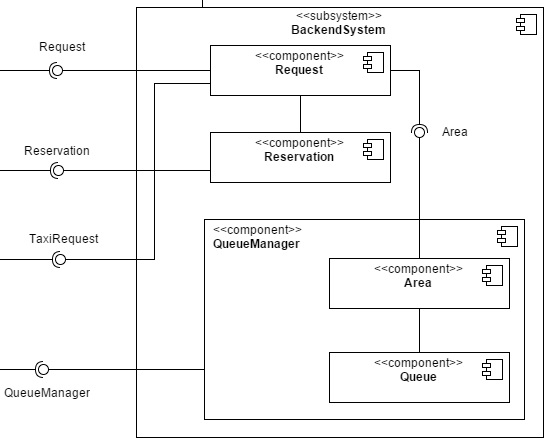
\includegraphics[width=1\linewidth]{../SE2_IMAGES/Backend}
			\caption{Backend components}
		\end{center}
	\end{figure}
	In this subsystem we have placed all the components (mainly entities) that we do not want to let the client
	interact directly. It is in direct communication with the frontend, responsible of the user
	management, and the database. This is practically the core of our system.
		\paragraph{Request}
		This is a stateful component. A User (Guest or RegisteredPassenger) can ask to create an instance
		which will be strictly related to the User himself and to the TaxiDriver who is asked to satisfy the
		request. A record in the database will be created to keep track of the operation, but when a taxi
		driver accepts or when the user closes the session, the request has no sense to exist anymore.
		In case a request is created automatically by a reservation, it will be related to the same user that booked it.
		\paragraph{Reservation}
		This is a stateful component. A RegisteredPassenger can ask to create an instance
		which will be strictly related to the User himself. A record in the database will be created to
		keep track of the operation, but when the User closes his session, the reservation has no sense to exist
		anymore. At the right time a job will be launched, creating a Request (even if the original instance
		does not exist anymore, the informations are stored in the database).
		\paragraph{QueueManager}
		This is a singleton component. Its interface is used by all the taxi drivers to interact with the areas and
		the queues. It is also responsible for the maintenance and the balancing of the queues.
		\paragraph{Area}
		This component is stateless. It is not connected to a single User, but, simply because it represents an Area,
		it has to serve all the users that require that area in the same way, there is no reason to relate the
		life of an area to the user's one. The main goal of this component is to manage the access to the one and
		only queue it contains.
		\paragraph{Queue}
		This is not truly an independent component, because we want to keep it strictly connected to the area,
		but we also want to be able to manage it without passing through the Area component all the times.
		It is easier fort he QueueManager to operate with a direct access to the queues.
		It is also sometimes useful to go back to areas from queues, so we keep a two way connection between them.
	\subsubsection{Database}
		\begin{figure}[h!]
			\begin{center}
				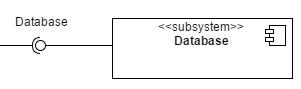
\includegraphics[scale=1]{../SE2_IMAGES/Database}
				\caption{Backend components}
			\end{center}
		\end{figure}
		\paragraph{Database} component is the database of our system. It stores all the important data that are often required by the Backend and the Frontend servers. Database component is singleton, it is created once and it is used during the whole life cycle of the system.
	\begin{landscape}
	\subsection{Deployment view}
	We provide a sight of how our components should be deployed in the various physical devices that compose the
	infrastructure of our system. In this case we assume that our Frontend and Backend subsystems run on the same
	server, so they are deployed in the same block. They could also be executed on different machines, the developer
	should simply define how the two subsystems should connect each other. On the application server will also
	be available the web pages accessible through a web browser.
		\begin{figure}[h!]
			\begin{center}
				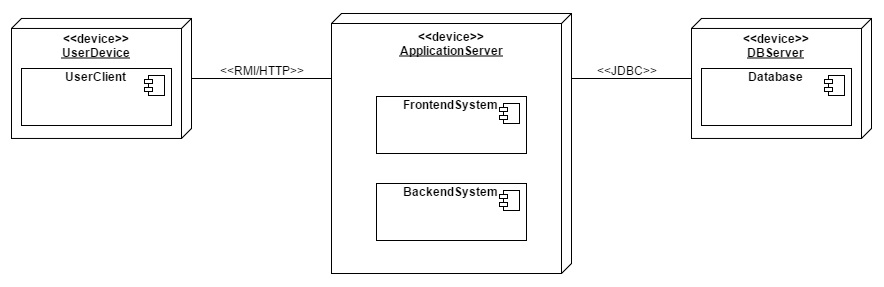
\includegraphics[width=0.9\linewidth]{../SE2_IMAGES/DeploymentDiagram}
				\caption{Deployment Diagram}
			\end{center}
		\end{figure}
	\end{landscape}
	\newpage
	\begin{landscape}
	\subsection{Runtime view}
	This is a "photograph" of the system during a hypothetical execution. The instances of the components and
	their interconnections are well visible inside the respective blocks where they are executed.
		\begin{figure}[h!]
			\begin{center}
				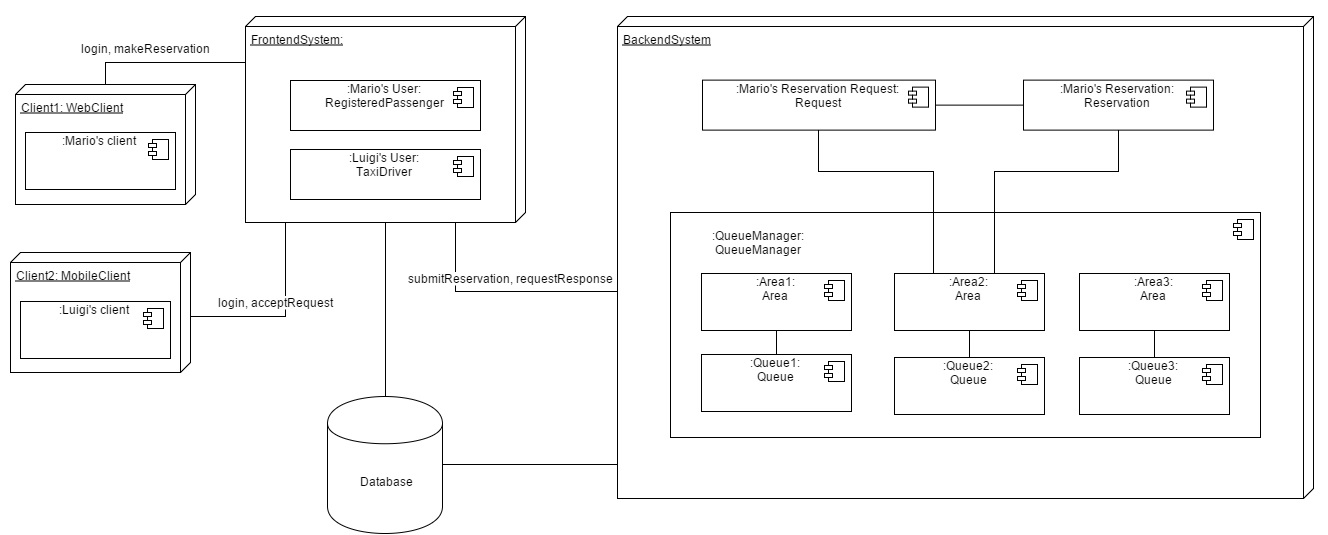
\includegraphics[width=0.9\linewidth]{../SE2_IMAGES/RuntimeDiagram}
				\caption{Runtime Diagram}
			\end{center}
		\end{figure}
	\end{landscape}
	\subsection{Sequence Diagrams}
	\label{subsec:Sequence Diagrams}
		\subsubsection{Guest submit request}
		This diagram shows how the system works when a user approaches the application a tries to submit
		a request as a guest user (not logged). We break the representation at the makeRequest method call
		because we will show how it works only one time in Figure~\ref{fig:makeRequest}.
		\begin{figure}[h!]
			\begin{center}
				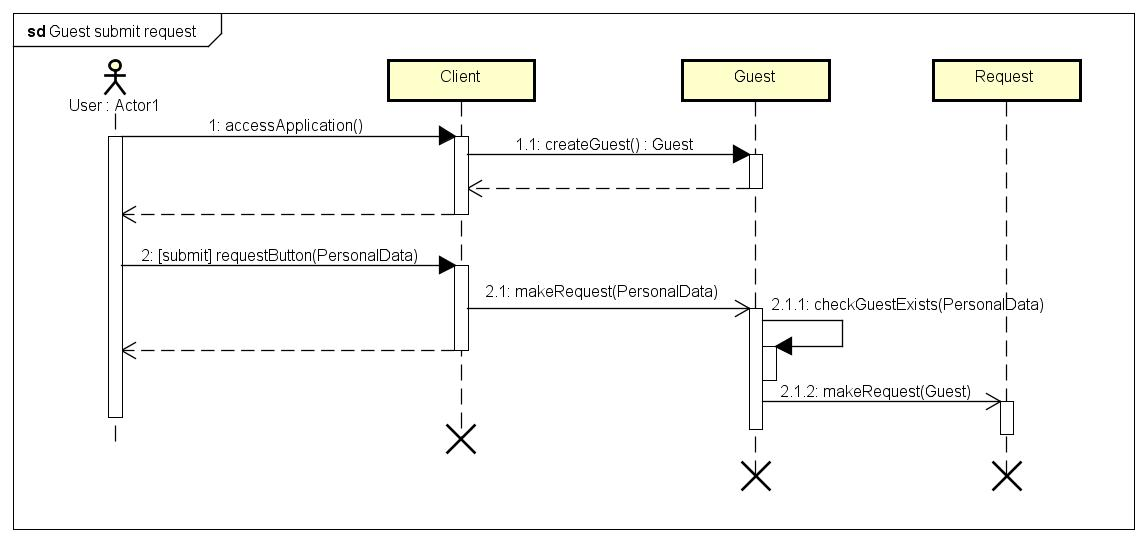
\includegraphics[width=1\linewidth]{../SE2_SD/GuestSubmitRequest}
				\caption{Guest submit request}
			\end{center}
		\end{figure}
		\clearpage
		\subsubsection{RegisteredPassenger submit request}
		This diagram shows the behaviour of the system when a registered passenger logs into the system (so
		we have also a sequence diagram example of the login process) and makes a reservation as a
		Registered Passenger. As before, we break the representation at the makeRequest method call
		because we will show how it works only one time in Figure~\ref{fig:makeRequest}.
		\begin{figure}[h!]
			\begin{center}
				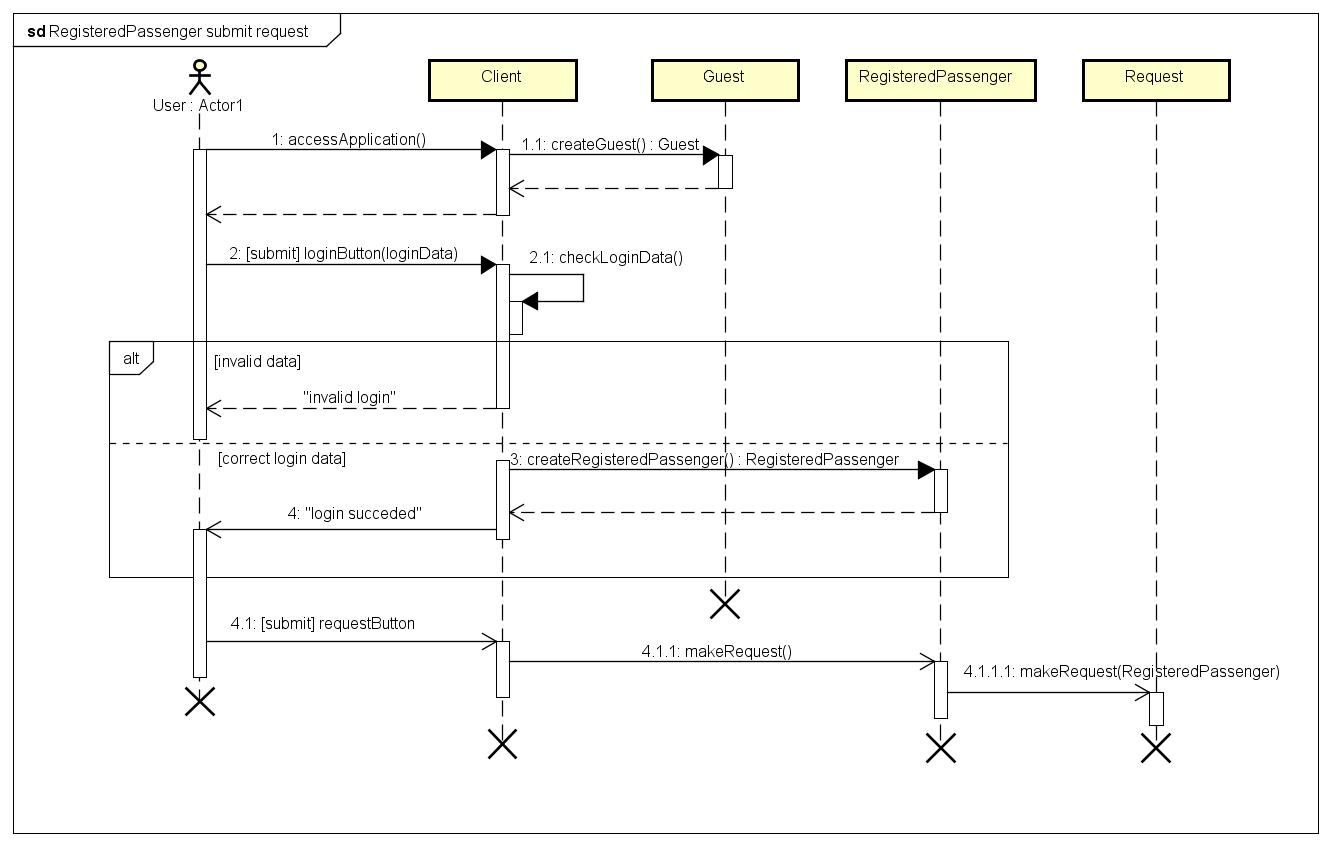
\includegraphics[width=1\linewidth]{../SE2_SD/RegisteredPassengerSubmitRequest}
				\caption{RegisteredPassenger submit request}
			\end{center}
		\end{figure}
		\clearpage
		\subsubsection{Make Request}
		This is how the system processes a Request submission.
		\begin{figure}[h!]
			\begin{center}
				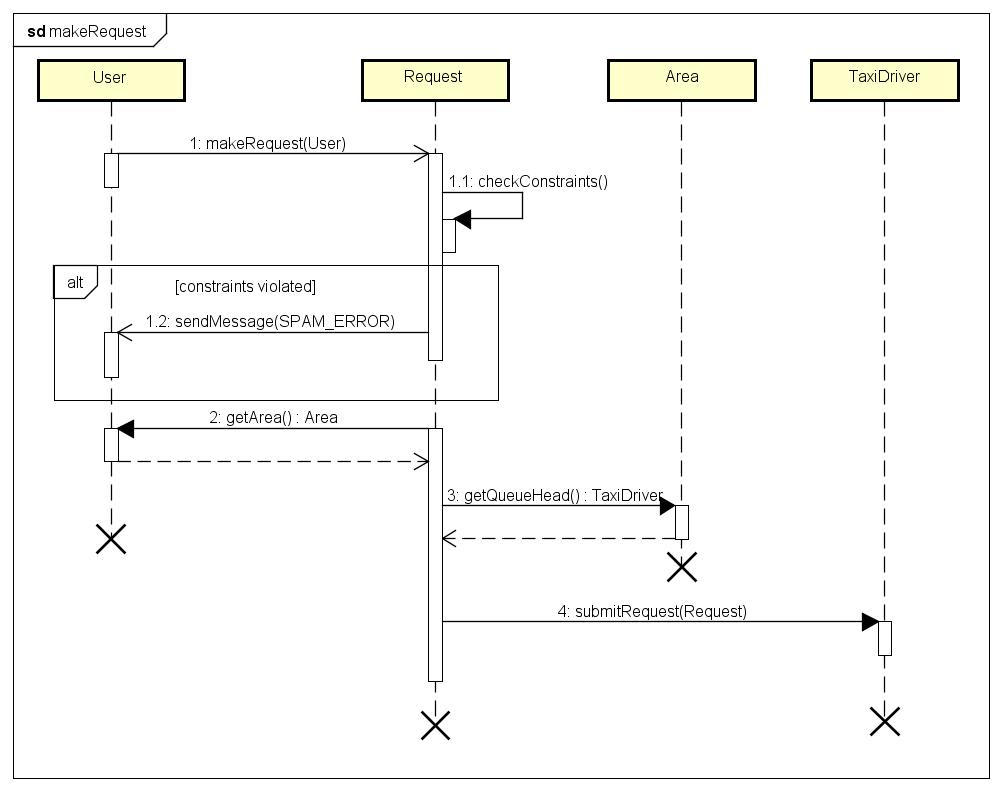
\includegraphics[width=1\linewidth]{../SE2_SD/makeRequest}
				\caption{Make Request}
				\label{fig:makeRequest}
			\end{center}
		\end{figure}
		\clearpage
		\subsubsection{Request response and Answer management}
		When a request has been created and the first notification is sent to a taxi, the system should
		manage the answer of the interested TaxiDriver bringing the necessary consequences to the Request
		(in order to finally satisfy it) and the TaxiDriver itself.
		\begin{figure}[h!]
			\begin{center}
				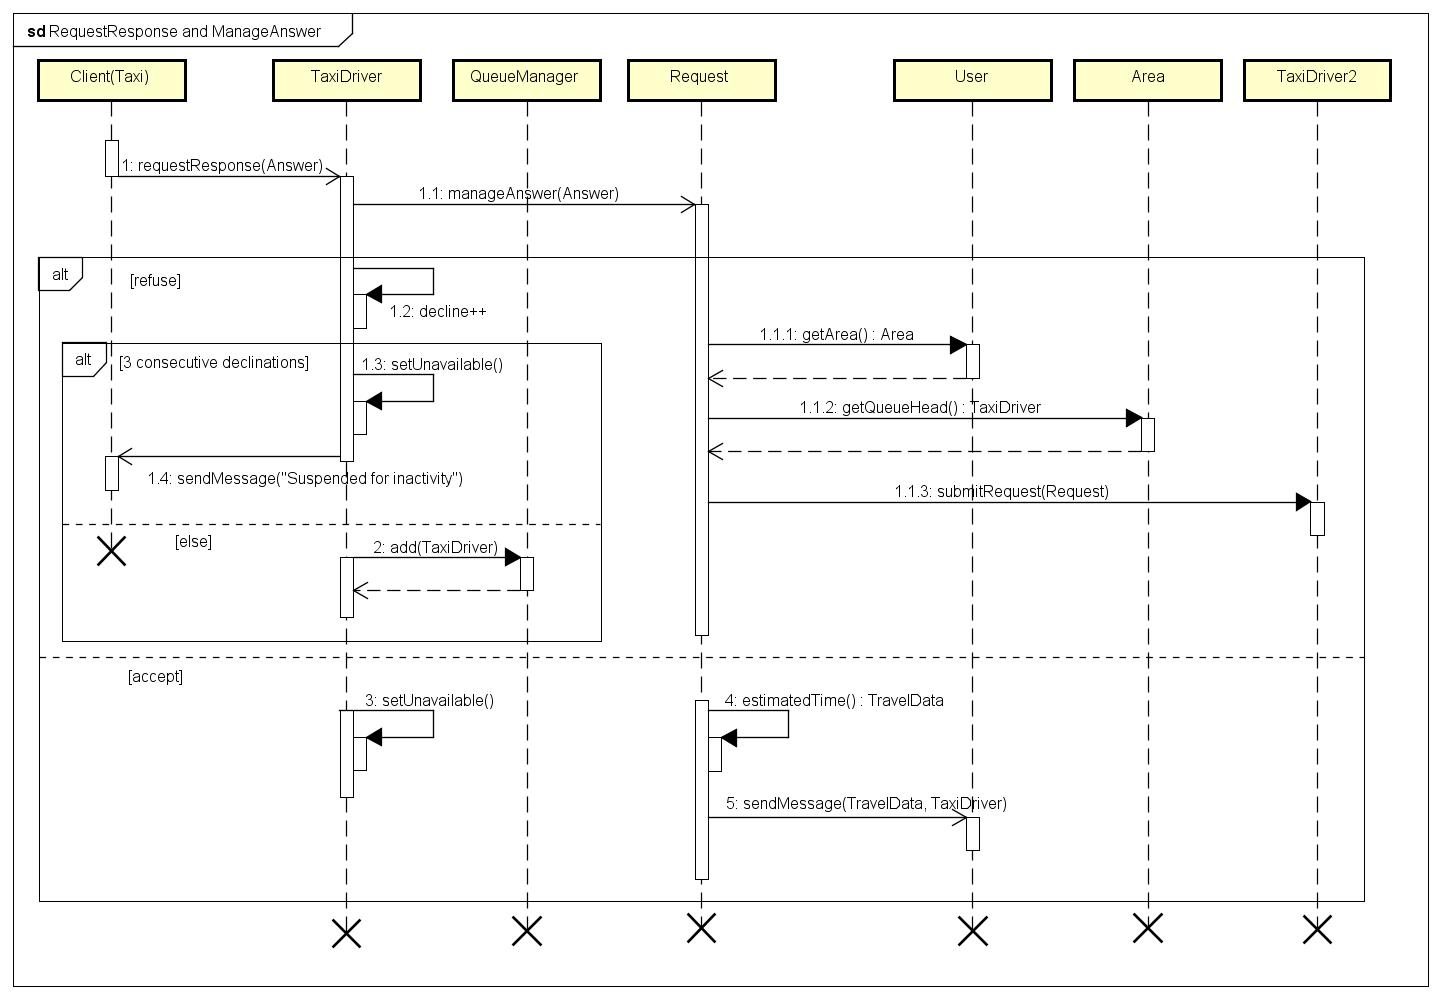
\includegraphics[width=1\linewidth]{../SE2_SD/RequestResponseManageAnswer}
				\caption{Request response and answer management}
			\end{center}
		\end{figure}
		\clearpage
		\subsubsection{Reservation}
		This is how the system processes a Request submission. As usual, we refer at the makeRequest
		diagram at Figure~\ref{fig:makeRequest} for the creation and management of the Request relative
		to this Reservation.
		\begin{figure}[h!]
			\begin{center}
				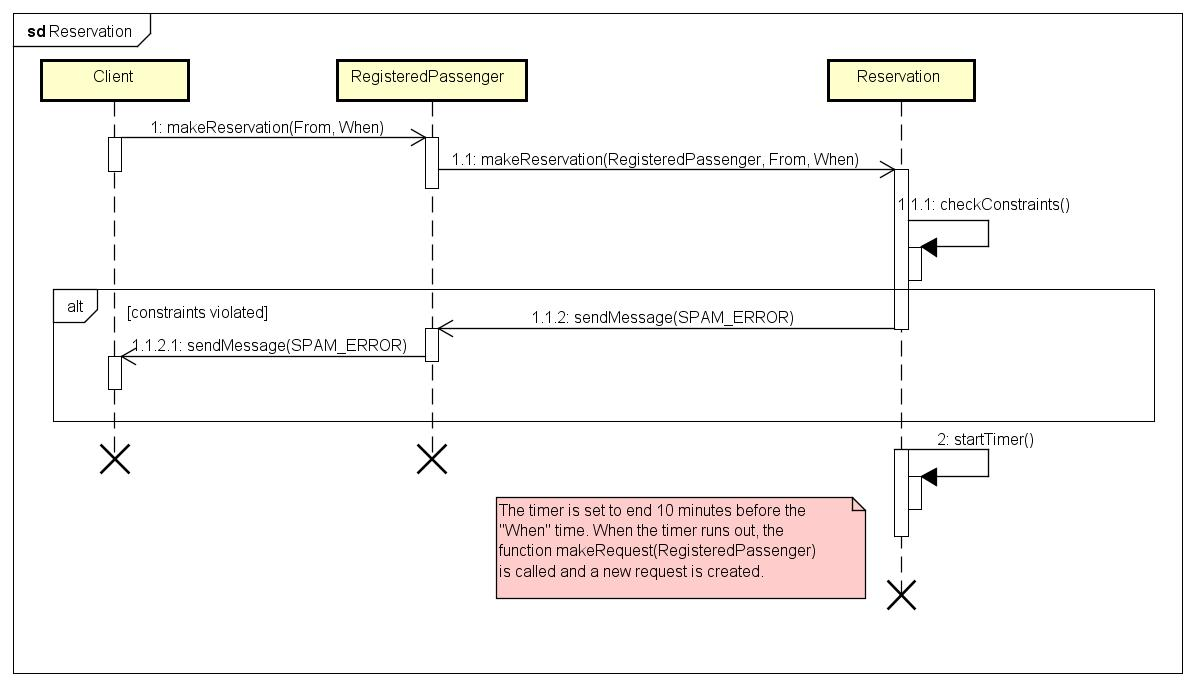
\includegraphics[width=1\linewidth]{../SE2_SD/Reservation}
				\caption{Reservation}
			\end{center}
		\end{figure}
		\clearpage
	\subsection{Component interfaces}
		\subsubsection{Guest}
		This is the basic interface assigned to client when the user accesses the application.
		It provides methods to perform all the operations that a "Guest" user can do:
		\begin{itemize}
			\item \textbf{register}: this method gives the possibility to an unregistered passenger to
			submit his personal data to perform a registration. If the registration succeeds, he will be
			stored in the database and will be able to log into the environment and be considered a registered passenger.
			\begin{description}
				\item[Input] Personal Data required for the registration
				\item[Output] The result of the registration (success or failure in case of error)
			\end{description}
			\item \textbf{login}: this method gives the possibility to login the environment to be considered
			a registered passenger. If this method succeeds, the Client will automatically substitute its Guest
			interface with a Registered Passenger interface related to the user that just performed the login.
			\begin{description}
				\item[Input] Login Data required for the login
				\item[Output] The result of the login (success or failure in case of error)
			\end{description}
			\item \textbf{makeRequest}: this method gives the possibility to a guest to make a single request.
			Some personal data and the consent for the automatic position recovery are required for the submission
			of the request. It also checks that all the constraints are respected before creating the Request object.
			\begin{description}
				\item[Input] Personal Data and consensus
				\item[Output] Nothing is returned directly, but the client will receive notifications about the
				request status.
			\end{description}
		\end{itemize}
		\subsubsection{RegisteredPassenger}
		This interface substitutes the Guest one in the client when the login is successfully completed.
		It provides all the	functionalities that a Registered Passenger can exploit.
		\begin{itemize}
			\item \textbf{makeRequest}: like in the Guest, this method gives the possibility to make a single request.
			No personal data is required for the submission, because the system will automatically use the
			informations stored in the database during the registration process. This method also checks that
			all the constraints are respected before creating the Request object.
			\begin{description}
				\item[Input] Nothing
				\item[Output] Nothing is returned directly, but the client will receive notifications about the
				request status.
			\end{description}
			\item \textbf{makeReservation}: this method gives the possibility to a logged user to make a single reservation.
			For a reservation some additional informations are required, that must be provided at the submission.
			This method also checks that all the constraints are respected before creating the Reservation object.
			\begin{description}
				\item[Input] The origin time and place where the taxi ride will begin
				\item[Output] Nothing is returned directly, but the client will receive notifications about the
				reservation and the consequent request statuses.
			\end{description}
			\item \textbf{deleteReservation}: this method gives the possibility to delete a reservation.
			The time constraints are checked and, if all the test are passed and no Request related to this
			reservation already exists, the record is deleted from the database. No Requests for this
			Reservation will be forwarded.
			\begin{description}
				\item[Input] The Reservation that has to be deleted
				\item[Output] Nothing is returned directly, but the client will receive notifications about the
				result of the operation.
			\end{description}
		\end{itemize}
		\subsubsection{TaxiDriver}
		This interface is provided by the TaxiDriver. With this interface a client is able to access the system via login. In particular this interface will be used only by mobile clients since the taxi drivers can't access the system via web. Once logged in they will be able to set themselves as available or unavailable and to see, accept or refuse requests.
		\begin{itemize}
			\item \textbf{login} this method gives the possibility to login the environment to be considered
			a taxi driver and will access the taxi driver interface
			\begin{description}
				\item[Input] Login Data required for the login
				\item[Output] The result of the login (success or failure in case of error)
			\end{description}
			\item \textbf{setAvailable} this method is used to change the taxi driver status to available
			\begin{description}
				\item[Input] Nothing
				\item[Output] Nothing is returned but the taxi driver will see on his application that his status has changed
			\end{description}
			\item \textbf{setUnavailable} this method is used to change the taxi driver status to unavailable
			\begin{description}
				\item[Input] Nothing
				\item[Output] Nothing is returned but the taxi driver will see on his application that his status has changed
			\end{description}
			\item \textbf{submitRequest} this method is used to send a request to a taxi driver
			\begin{description}
				\item[Input] Request that will be sent to the taxi driver
				\item[Output] The result of the submit (success or failure in case of error)
			\end{description}
		\end{itemize}
		\subsubsection{Request}
		This interface is provided to the User instances to create, and eventually interact, with a request.
		\begin{itemize}
			\item \textbf{makeRequest}: this method receives a User (a Guest o a RegisteredPassenger instance)
			and creates	an instance of a Request, launching also all the necessary processes to satisfy it.
			\begin{description}
				\item[Input] User
				\item[Output] A Request instance
			\end{description}
		\end{itemize}
		\subsubsection{Reservation}
		This interface is provided to the User instances to create, and eventually interact, with a reservation.
		\begin{itemize}
			\item \textbf{makeReservation}: this method receives a User (a Guest o a RegisteredPassenger instance)
			and the place and time informations necessary for the creation of a Reservation and instances a
			Reservation object, launching also all the necessary processes to satisfy it. This method fundamentally
			launches the makeRequest functionality at the right time.
			\begin{description}
				\item[Input] User, When and Where the request will take place
				\item[Output] A Reservation
			\end{description}
		\end{itemize}
		\subsubsection{TaxiRequest} 
		This interface is provided by the Request. With this interface TaxiDrivers receive requests that they can accept or refuse them.
		\begin{itemize}
			\item \textbf{requestReply} this method is used by the taxi driver to accept or refuse the request they have received
			\begin{description}
				\item[Input] Request that the taxi driver has received and his answer
				\item[Output] The result of the reply (success or failure in case of error)
			\end{description}
		\end{itemize}
		\subsubsection{QueueManager} 
		This interface is provided by the QueueManager. With this interface TaxiDrivers can set their status as available or unavailable, affecting their presence in the queue. This also mean that the QueueManager can add or remove a TaxiDriver from the queue.
		\begin{itemize}
			\item \textbf{add} this method is used by the QueueManager to add a taxi driver to a queue
			\begin{description}
				\item[Input] TaxiDriver that will be added to the queue
				\item[Output] the result of the operation (success or failure in case of error)
			\end{description}
			\item \textbf{remove} this method is used to remove a taxi driver from a queue
			\begin{description}
				\item[Input] TaxiDriver that will be removed from the queue
				\item[Output] the result of the operation (success or failure in case of error)
			\end{description}
		\end{itemize}
		\subsubsection{Area} 
		This interface is provided by the Area. With this interface the Request can retrieve Area's informations and get the first available taxi from queue in order to submit him a request.
		\begin{itemize}
			\item \textbf{getQueueHead} this method is used to retrieve the first taxi in a queue
			\begin{description}
				\item[Input] Nothing
				\item[Output] The first taxi driver from the queue corresponding to the area in use
			\end{description}
		\end{itemize}
		\subsubsection{Database} 
		This interface is provided by the database and it is used by the Backend and Frontend servers. With this interfaces Backend and Frontend servers are able to interact with the database, storing and retrieving data about for example registered passengers or reservations. There is no particular function since it will depend on how the database is effectively implemented.
	\newpage
	\subsection{Architectural styles and patterns}
	We want suggest some some styles and patterns that we decided to adopt in our system, but that have not been explained
	clearly yet.
	\begin{itemize}
		\item The first, and probably the most relevant, is the four tier architecture. Our system is designed to
		support a JEE architecture with a thin client on the user device, which is used only as a interface, and a,
		relatively, fat server that processes all the operations.
		\item An MVC approach has been followed. The user interfaces in the UserClient (view) are used only for
		data exploration and command submission by the user.
		The backend operates and processes (controller) the requests coming	from the user interfaces and interacts
		with the persistent and dynamic (but global, like areas and queues)	data belonging to the model.
		\item JMS is a good way to solve the "messaging problem". JMS is a services provided by JEE in its architecture.
		Its goal is to manage the point-to-point message delivery in an asynchronous way, simply specifying who
		has to receive a notification. A similar approach can be reproduced also without the JMS constraint.
		\item There are two patterns that could be useful during implementation:
		\begin{description}
			\item[Factory Method] useful for components that must be continuously created,
			maybe also by different components or as a result of different commands, like Users (Guest, ecc.),
			Requests and Reservations. This allows a stronger control on the instance creation.
			\item[Singleton] useful for components which needs only one instance in the whole system.
		\end{description}
	\end{itemize}
	
	
\section{Algorithm Design}
	In this section are presented some algorithms that we consider fundamental to understand how
	our system should work. We will not provide the code of the most common functionalities, but we
	have selected two of the most significant for our project.
	\subsection{Request management}
	This algorithm is focused on the request managment.\\ In the first procedure ManageRequest, first it checks if the request by that specific client is valid, meaning that the client hasn't done any request in the last 30 minutes. If the request is not valid then it is refused with an error notification sent to the client, otherwise the request is instantiated and stored in the database. From the request's info it retrieves an area and then the first taxi available, to which the request is sent.\\ In the second procedure SubmitRequest there's a timer indicating the window of time that the taxi driver has to answer the request and the notification that is showed to the taxi driver.\\ In the third procedure RequestReply it is checked the answer given by the taxi driver. In case of negative answer, the number of declined answers by that taxi driver in incremented by 1 and when it reaches the third consecutive decline the taxi is set unavailable, otherwise it is added in queue again.\\ In the last procedure ManageAnswer it is checked again the answer. In case of negative answer the operations to retrieve the first taxi in the queue are done again, otherwise the request confirmation is sent to the client which contains the estimated arrival time and the taxi ID.
	\subsubsection{Pseudocode}
	\begin{algorithm}
		\begin{algorithmic}[1]
			\Procedure {MakeRequest}{user}
			\If {$!validRequest(user)$}
			\State $sendMessage(SPAM\_REQUEST\_ERROR, user)$
			\Else
			\State {$rqst \gets new\  Request(user)$}
			\State {$storeRequest(rqst)$}
			\State {$area \gets retrieveArea(origin)$}
			\State {$taxi \gets area.queue.remove(0)$}
			\State {$taxi.submitRequest(rqst)$}
			\EndIf
			\EndProcedure
		\end{algorithmic}
	\end{algorithm}
	\begin{algorithm}
		\begin{algorithmic}[1]
			\Procedure {SubmitRequest}{request}
			\State {$timer \gets new Timer(60)$}
			\State {$timer.start()$}
			\State {$sendMessage(rqst, taxi)$}
			\EndProcedure
		\end{algorithmic}
	\end{algorithm}
	\begin{algorithm}
		\begin{algorithmic}[1]
			\Procedure {RequestResponse} {answer, request}
			\State{$request.manageAnswer(answer)$}
			\If {$answer \equiv REFUSE$}
			\State{$ taxi.declined++ $}
			\If{$ taxi.declined \equiv 3 $}
			\State {$ taxi.setUnavailable() $}
			\Else
			\State{$ queueManager.add(taxi) $}
			\EndIf
			\Else
			\State {$ taxi.setUnavailable() $}
			\EndIf
			\EndProcedure
		\end{algorithmic}
	\end{algorithm}
	\begin{algorithm}
		\begin{algorithmic}[1]
			\Procedure {ManageAnswer}{answer}
			\If{$ answer \equiv REFUSE $}
			\State{$area \gets retrieveArea(rqst.origin)$}
			\State{$taxi \gets area.queue.remove(0)$}
			\State{$taxi.submitRequest(rqst)$}
			\Else
			\State {$user.sendConfirmation(estimatedTime(), taxi)$}
			\EndIf
			\EndProcedure
		\end{algorithmic}
	\end{algorithm}
	\clearpage
	\subsection{Queue balancing}
	This algorithm shows the mechanism that every two minutes balances the area queues.
	The idea is that a taxi may move from its position at any time, for any reason, and, perhaps,
	pass through other areas than the one he belonged to when he was first inserted into the system.
	So a simple job running this algorithm can keep the system up to date and avoid inconsistencies
	(like sending a notification to a taxi out of the interested area).
		\subsubsection{Pseudocode}
		\begin{algorithm}
			\begin{algorithmic}[1]
				\ForAll {$TaxiDrivers\textnormal{ available as }TaxiDriver$}
					\State $actualArea \gets TaxiDriver.Area$
					\State $oldArea \gets TaxiDriver.Queue.Area$
					\If{$actualArea \neq oldArea$}
						\State $oldArea.\textnormal{extract}(TaxiDriver)$
						\State $actualArea.\textnormal{insert}(TaxiDriver)$
					\EndIf
				\EndFor
				\State $criticalAreas \gets \textnormal{List}$
				\ForAll{$Areas \textnormal{ as } Area$}
					\If{$Area.Queue.size \leq Area.minCriticalSize$} 
						\State $criticalAreas.\textnormal{add}(Area)$
					\EndIf
				\EndFor
				\State $surplusTaxis \gets \textnormal{List}$
				\ForAll{$Queues \textnormal{ as } Queue$}
					\ForAll{$TaxiDrivers \textnormal{ with index } \geq Queue.Area.maxCriticalSize$}
						\State $surplusTaxis.\textnormal{add}(TaxiDriver)$
					\EndFor
				\EndFor
				\State $nofitication \gets$ "In the areas ".$criticalAreas$.toString()." we have a taxi shortage.
					Go there and get back to work!"
				\ForAll {$surplusTaxis \textnormal{ as } TaxiDriver$}
					\State $TaxiDriver.\textnormal{sendNotification}(notification)$
				\EndFor
			\end{algorithmic}
		\end{algorithm}
		\subsubsection{Clarifications}
		The first section of the algorithm updates the area queues, moving taxis from the areas they belonged last
		time they were inserted to the one they belong now, only if they are different (we assume that
		\textit{TaxiDriver.Area} retrieves the actual position of the taxi and returns the corresponding area).
		After the update, the system tries to balance his queues where the values are out of some critical values.
		It is simple: if the length of an area queue is under a \textit{minCricitalSize}, that area needs to be
		"filled" with taxis. If the length of an area queue is above a \textit{maxCricitalSize}, that area has
		too many taxis without a reason an the last taxis in those queues can be moved elsewhere.
		So the system notifies these \textit{surplusTaxis}, advising them to move where they are really needed.
\section{User Interface Design}
\subsection{User Experience}
\subsubsection{Traditional User}
\begin{figure}[h!]
	\begin{center}
		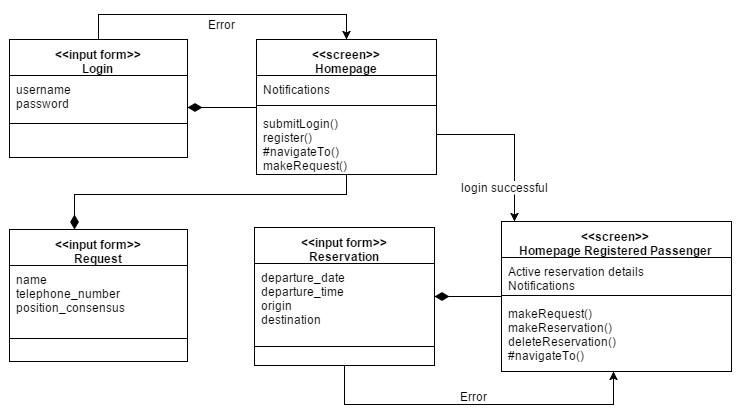
\includegraphics[width=1\linewidth]{../SE2_IMAGES/UserUX}
		\caption{Component Diagram}
	\end{center}
\end{figure}
\newpage
\subsubsection{Taxi Driver}
\begin{figure}[h!]
	\begin{center}
		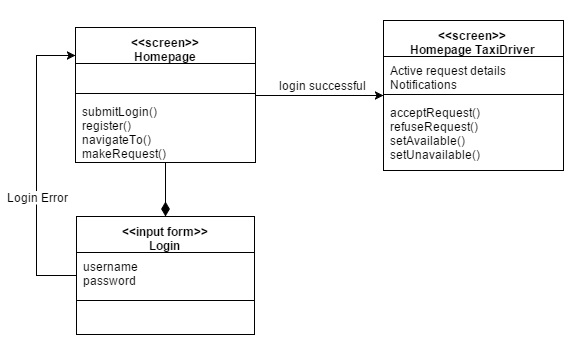
\includegraphics[width=1\linewidth]{../SE2_IMAGES/TaxiUX}
		\caption{Component Diagram}
	\end{center}
\end{figure}
\section{Requirements Traceability}
In this section we will go over how what is written in the Specific Requirements section in the RASD is connected to some design element defined in this document.
\subsection{Functional Requirements}
The functional requirements that are present in the RASD are connected first of all to our component view, in which it is clear where each requirement is satisfied and by which component (make reference to subsection~\ref{subsec:High Level Components and their interaction} , and also better explained in section~\ref{subsec:Sequence Diagrams} . They are also present in the sequence diagrams showing even more in details some functionality.
\subsection{API}
The API of GoogleMaps are used by the components of the Backend system, in particular by the Area. The main application is retrieving the taxi position and then assign that taxi to the correct area, but also calculating the estimated time of arrival of a taxi to the origin position of a request. 

\section{References}
In order to write this Design Document we use as reference:
\begin{itemize}
	\item \textit{IEEE standard on Design Descriptions}
	\item \textit{IEEE 1417}
	\item \textit{Other Design Documents}
\end{itemize}

\end{document}